\subsection{Virtual heart model}
\label{heartmodel}

Since we don't have access to real human hearts for testing, we have developed a \emph{Virtual Heart Model (VHM)}, which simulates the \emph{timing aspects} of the operation of a human heart, and ignores other physiological details.
\todo[inline]{ZJ : review following for accuracy}
The VHM models each of the following heart structures as a Finite State Machine (FSM): the SA node, the AV node, and the ventricle.
The paths connecting them are also modeled as FSMs.
These FSMs capture the operating modes of the nodes (depolarizing, refractory, idle, etc.) and those of the paths (conducting, backward-conducting, etc.), as well as the conditions leading from one state to another (e.g. a path conduction is followed by the node entering the depolarized state).
See Fig.~\ref{fig:FSMSA} for an example of a node FSM.
\begin{figure}[t]
\centering
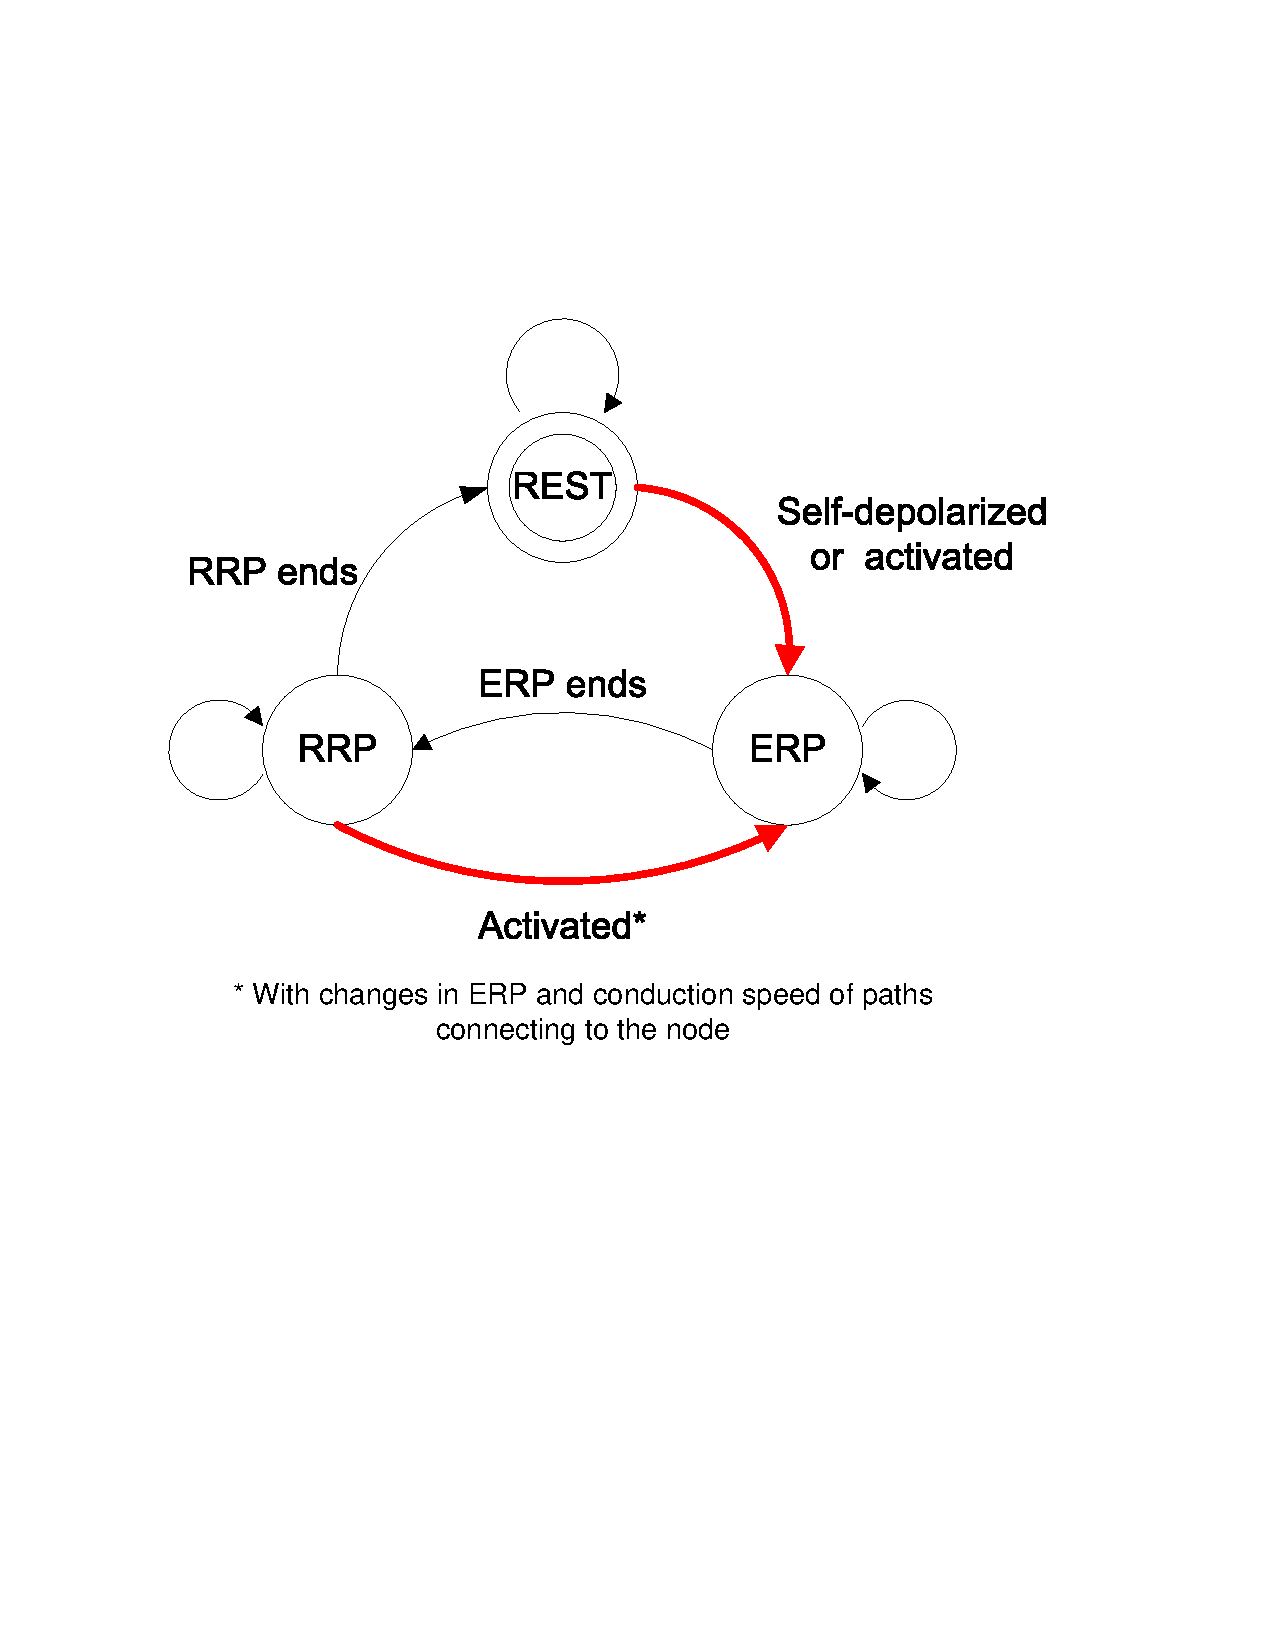
\includegraphics[scale=0.2]{node_automata.pdf}
\caption{FSM modeling the SA node showing Effective and Relative Refractory Periods (ERP and RRP) and the Rest state.}
\label{fig:FSMSA}
\end{figure}
The VHM is implemented in both Simulink and Matlab. 
We used the VHM to simulate different heart conditions in a closed loop with the pacemaker model, such as Wenckebach AV nodal response, atrial flutter and pacemaker mediated tachycardia.
The VHM functional output has been validated by the director of cardiac electrophysiology in the Philadelphia VA Hospital and by electrophysiologists in the Hospital of the University of Pennsylvania. 
More details are available in \cite{Jiang1}\cite{vhm_iccps11}\cite{embc10}.
